%\documentclass[a4paper]{article}
\usepackage[utf8]{inputenc}
\usepackage[spanish, es-tabla, es-noshorthands]{babel}
\usepackage[table,xcdraw]{xcolor}
\usepackage[a4paper, footnotesep = 1cm, width=20cm, top=2.5cm, height=25cm, textwidth=18cm, textheight=25cm]{geometry}
%\geometry{showframe}

\usepackage{tikz}
\usepackage{amsmath}
\usepackage{amsfonts}
\usepackage{amssymb}
\usepackage{float}
\usepackage{graphicx}
\usepackage{caption}
\usepackage{subcaption}
\usepackage{multicol}
\usepackage{multirow}
\setlength{\doublerulesep}{\arrayrulewidth}
\usepackage{booktabs}

\usepackage{hyperref}
\hypersetup{
    colorlinks=true,
    linkcolor=blue,
    filecolor=magenta,      
    urlcolor=blue,
    citecolor=blue,    
}

\newcommand{\quotes}[1]{``#1''}
\usepackage{array}
\newcolumntype{C}[1]{>{\centering\let\newline\\\arraybackslash\hspace{0pt}}m{#1}}
\usepackage[american]{circuitikz}
\usetikzlibrary{calc}
\usepackage{fancyhdr}
\usepackage{units} 

\graphicspath{{../Calculos-Potencia/}{../Caracteristicas/}{../Consideraciones/}{../Gain-Stage/}{../Input-Stage/}{../Output-Stage/}{../Simulaciones/}{../Alimentacion/}{../Conclusiones/}}

\pagestyle{fancy}
\fancyhf{}
\lhead{22.12 Electrónica II}
\rhead{Mechoulam, Lambertucci, Rodriguez, Londero, Scala}
\rfoot{Página \thepage}
%
%\begin{document}

\subsection{Introducción}
La etapa de amplificación de tensión (o VAS) a menudo es considerada como la etapa más crítica de un amplificador de potencia , dado que no solo provee la ganancia de tensión sino que también debe manejar todo el rango de la tensión de salida. Esto indicaría que puede jugar un rol significativo en la distorsión armónica de la señal, sin embargo un VAS bien diseñado contribuye relativamente poco a la distorsión total, e incluso si se tomasen pasos extra para intentar linealizar aún más la salida, estas contribuciones comparadas con las hechas en una etapa de entrada, son completamente despreciables.\\
\subsection{Diseños propuestos}
El primer diseño que se pensó fue un emisor común que se observa a continuación que si bien  cuenta con varios problemas estos van  a ser sorteados en las siguientes lineas.
\begin{figure}[H]
\centering
	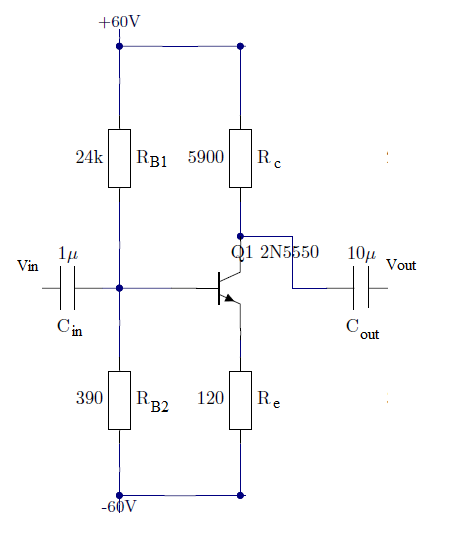
\includegraphics[width=0.5\textwidth]{ImagenesGain-Stage/ec1.png}
	\caption{Primer diseño Emisor Común}
	\label{fig:ec1}
\end{figure}

El primer problema que se afrontó fue el de limitar la ganancia de altas frecuencias.
Para esto se introduce una linea de realimentación negativa utilizando $C_{dom}$ el cual limita la ganancia de altas frecuencia y así asegura mayor estabilidad.
 \begin{figure}[H]
\centering
	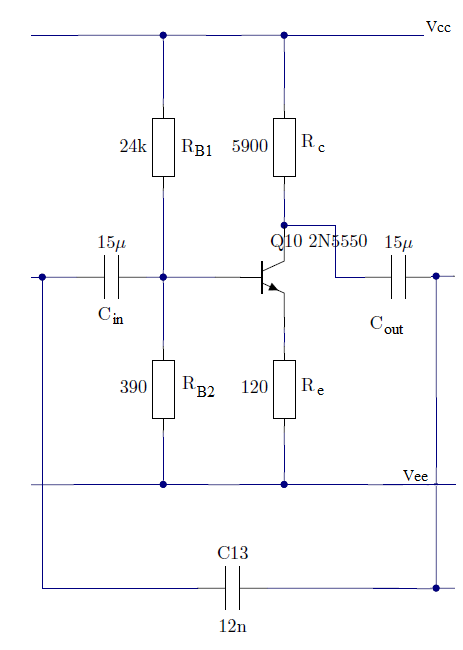
\includegraphics[width=0.5\textwidth]{ImagenesGain-Stage/ec2.png}
	\caption{Segundo diseño Emisor Común}
	\label{fig:ec2}
\end{figure}
En cuanto al cálculo de $C_{in}$ o $C_{out}$ se buscó que la impedancia para frecuencias medias sea despreciable frente a la impedancia vista desde el colector o la base.

Para el caso de $C_{Dom}$ se eligió un valor tal que las altas frecuencias vean un camino de baja impedancia comparado con la entrada del emisor común. De esta manera, las frecuencias altas no serán amplificadas.

Es importante que la ganancia a lazo abierto del VAS sea alta, así este puede ser linealizado. Si se intenta aumentar la ganancia del emisor común, se sabe que la ganancia de este está descripto por la ecuación:
\begin{align}
A_{vs}=\frac{-R_D}{R_E}
\end{align}

Si se quiere subir la ganancia, puede subirse el valor de $R_C$, pero esto dado una $I_c$ determinada por la  malla de entrada, provocará que caiga más tensión sobre la resistencia $R_C$ y así consuma un valor de potencia mucho más elevado. Una manera de asegurar una gran ganancia es utilizar una carga activa con una fuente de corriente, así suministrando la corriente necesaria, y mostrando una alta impedancia.

Además, se optó por utilizar un acople por fuente de corriente en vez de uno capacitivo con la idea de no introducir singularidades no deseadas en el circuito.
 \begin{figure}[H]
\centering
	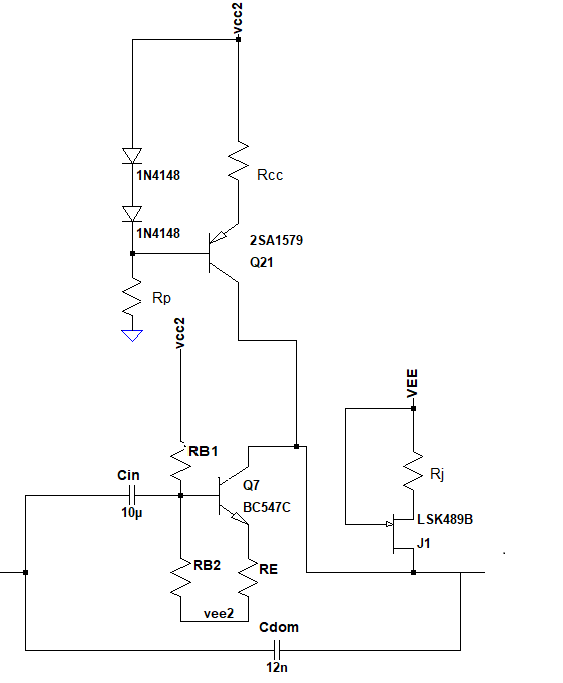
\includegraphics[width=0.5\textwidth]{ImagenesGain-Stage/ec3.png}
	\caption{Tercer diseño Emisor Común}
	\label{fig:ec3}
\end{figure}

Para la fuente de corriente de la carga activa se optó por utilizar una fuente compensada. Mientras que para el acople se utilizó una fuente implementada con JFET, debido a que en esa zona el circuito tiene la máxima variación de tensión, lo cual si se hubiese implementado con una fuente con BJT podría tener problemas de Saturación / Corte.\\
El transistor se le impuso una tensión de $V_{ce}$ de $\frac{V_{cc}+V_{ee}}{2}$ al igual que un valor de corriente $I_c = 10 \ mA$, al igual que optar por una resistencia de emisor baja.\\
Los valores utilizados para el circuito responden a las siguientes ecuaciones:
\begin{align}
R_{B2}= \frac{V{Re}+V_{be}}{I_{RB}} \approx 390 \ \Omega |_{IRb=5 \ mA \  \ \wedge \ \  Vre=1.2 \ V}
\end{align}
\begin{align}
R_E=\frac{I_{Rb}\cdot R_{B2}-2V_{be}}{I_c}=120 \ \Omega
\end{align}
\begin{align}
R_{B1}= \frac{V_{cc}+V_{ee}-I_{Rb}\cdot R_{B2} }{I_{Rb}}=24 \ k\Omega
\end{align}
Luego para la fuente compensada se obtuvo un valor para la resistencia $R_{cc}$, tal que suministre los $10 \ mA$ al colector del transistor.

\begin{align}
R_{cc}=\frac{V_{be}}{I_c}\approx 76 \ \Omega
\end{align}
También se obtiene el parámetro de la impedancia de salida de la fuente compensada la cual es de aproximadamente:
\begin{align}
R_{of} = (R_cc // hie^*)+(1+hfe^* )\cdot rce
\end{align}

En cuanto a la compensación por corriente se optó por el transistor \href{https://ar.mouser.com/datasheet/2/827/DS_UJ3N065080K3S-1530401.pdf}{UJ3N065080K3S} debido a que puede manejar el rango de tensiones de la salida y puede proveer una corriente suficiente, si bien este era el transistor ideal, el subcircuito encontrado en linea parece no funcionar correctamente por lo que se utilizo el \href{http://www.linearsystems.com/lsdata/datasheets/LSK489_LOW_NOISE,_LOW_CAPACITANCE_MONOLITHIC_DUAL_N-CHANNEL_JFET.pdf}{LSK489B} para la simulación, pero ese transistor sería el utilizado en la realidad. En cuanto a la  elección de la resistencia del Jfet, se consideraron los parámetros $V_p$, $I_{dss}$.
\begin{align}
I_D=-\frac{V_{GS}}{R_j}
\end{align}
El valor de la corriente de drain que se necesitará será la corriente la cual se fugaría del VAS hacia la etapa de salida al no estar presente el capacitor, la cual es de un valor de aproximadamente $5 \ mA$.
\begin{align}
I_D= I_{DSS} \cdot \left(1-\frac{V_{GS}}{V_P} \right)^2
\end{align}

De aquí se obtiene $R_j \approx 65 \ \Omega$. La fuente de corriente de acople posee además una segunda característica. Esta permite no solo regular el nivel de continua de reposo a la salida de cada clase AB, sino también el nivel de continua de reposo sobre la carga. Basta que ambas salidas en reposo sean iguales para que la continua de reposo sobre la carga sea nula, sin embargo, si no se compensa correctamente con esta fuente el nivel de continua en reposo a la salida de cada clase AB, se consumirá una gran potencia lo que disminuirá considerablemente el rendimiento del amplificador, por más que los parlantes no se dañen debido a la simetría del circuito.

Como última consideración se optó por poner 3 etapas amplificadoras como la de la Figura (\ref{fig:ec1}) previo al diseño de la Figura (\ref{fig:ec3}) con la intención de aumentar la ganancia del bloque A tal  que valga que $\alpha \cdot \beta \gg 1$ dado que $\beta$ será de un valor muy pequeño para lograr llegar a disipar como máximo $1.5 \ kW$ sobre la carga.
Con esto dicho la tension sobre los $V_{ce}$ serán:\\
Para el transisitor con carga activa:
\begin{align}
V_{ce-ec-rms}= V_{ce-cc}+\frac{ \hat{V_o}}{\sqrt{2}}\approx 68.9V 
\end{align}
Para la carga activa será:
\begin{align}
V_{ce-load-rms}= V_{cc}-I_C-\frac{\hat{V_{ce-ec}}}{\sqrt{2}}\approx 71.5V
\end{align}


%\begin{align}
%\end{align}
%\end{document}
